%%%% APÊNDICE A
%%
%% Texto ou documento elaborado pelo autor, a fim de complementar sua argumentação, sem prejuízo da unidade nuclear do trabalho.

%% Título e rótulo de apêndice (rótulos não devem conter caracteres especiais, acentuados ou cedilha)
\chapter{User App Screenshots}\label{ap:userapp}

\begin{figure}[H]
	\centering
	\caption[Product listing and subtotal]{Product listing and subtotal}
	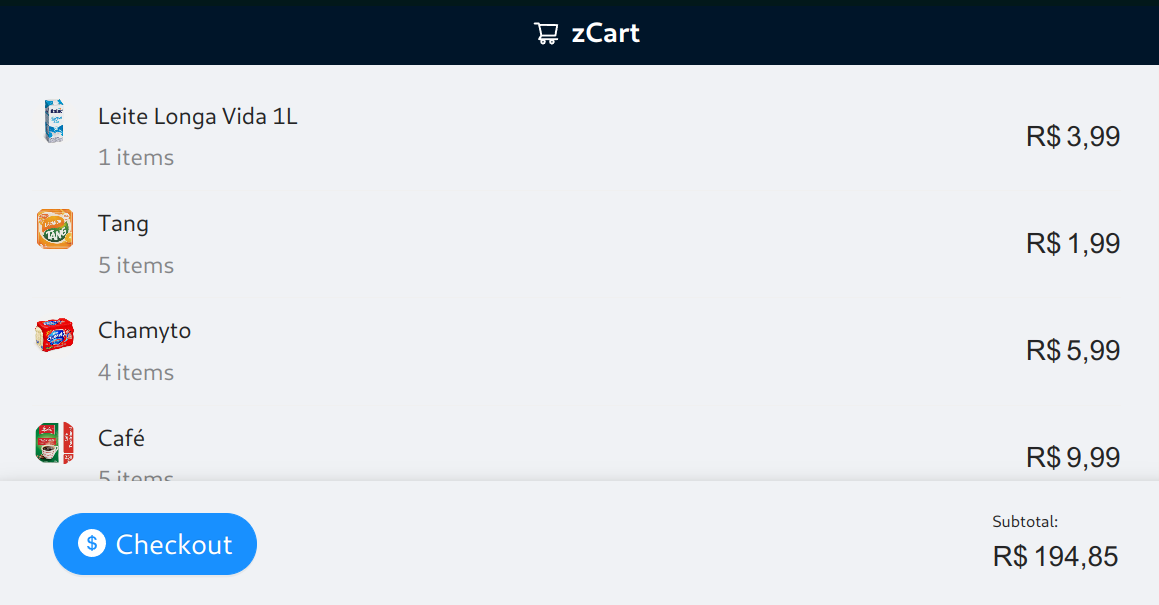
\includegraphics[width=1\textwidth]{./images/userapp.png}
    \fonte{}
\end{figure}

\begin{figure}[H]
	\centering
	\caption[Item addition notification]{Item addition notification}
	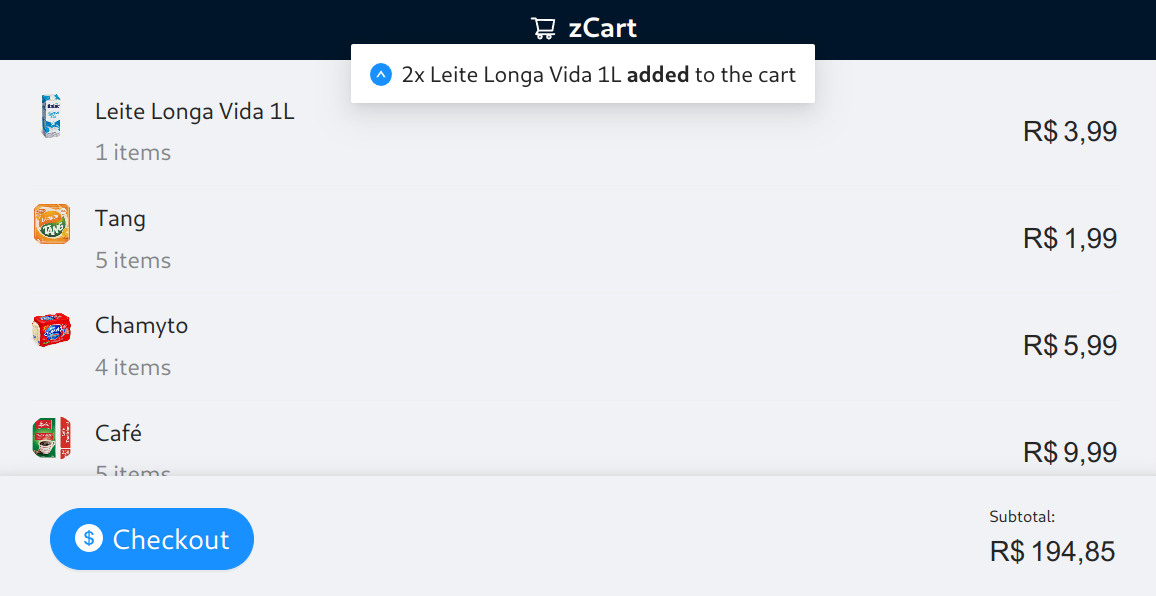
\includegraphics[width=1\textwidth]{./images/userapp2.png}
    \fonte{}
\end{figure}

\begin{figure}[H]
	\centering
	\caption[Item removal notification]{Item removal notification}
	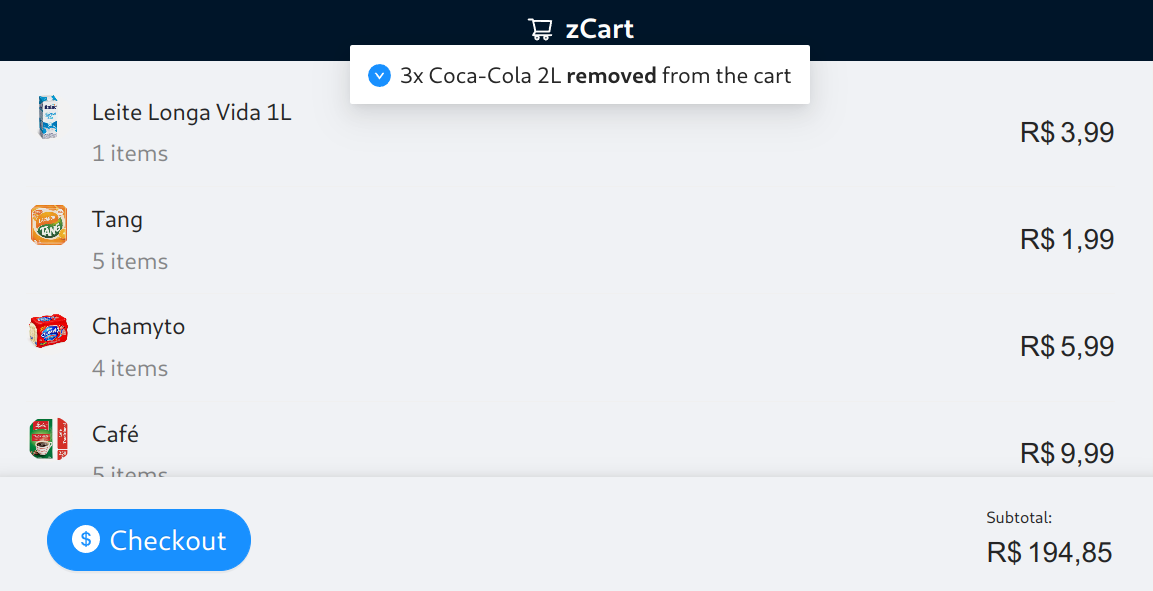
\includegraphics[width=1\textwidth]{./images/userapp3.png}
    \fonte{}
\end{figure}

\begin{figure}[H]
	\centering
	\caption[Pre-checkout confirmation popup]{Pre-checkout confirmation popup}
	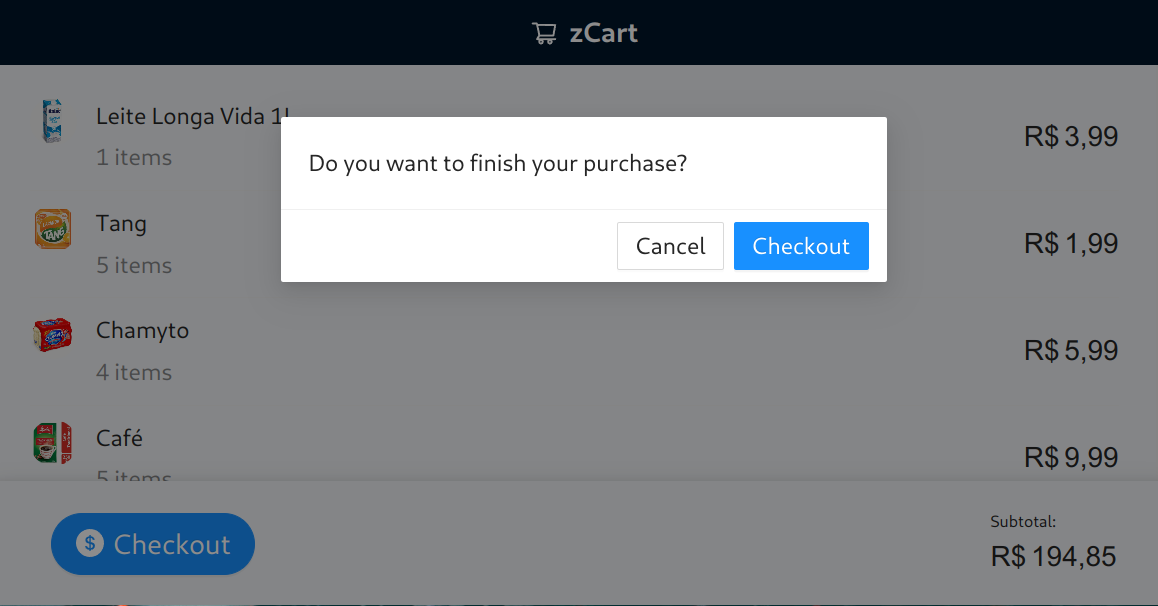
\includegraphics[width=1\textwidth]{./images/userapp4.png}
    \fonte{}
\end{figure}

\begin{figure}[H]
	\centering
	\caption[Post checkout screen]{Post checkout screen}
	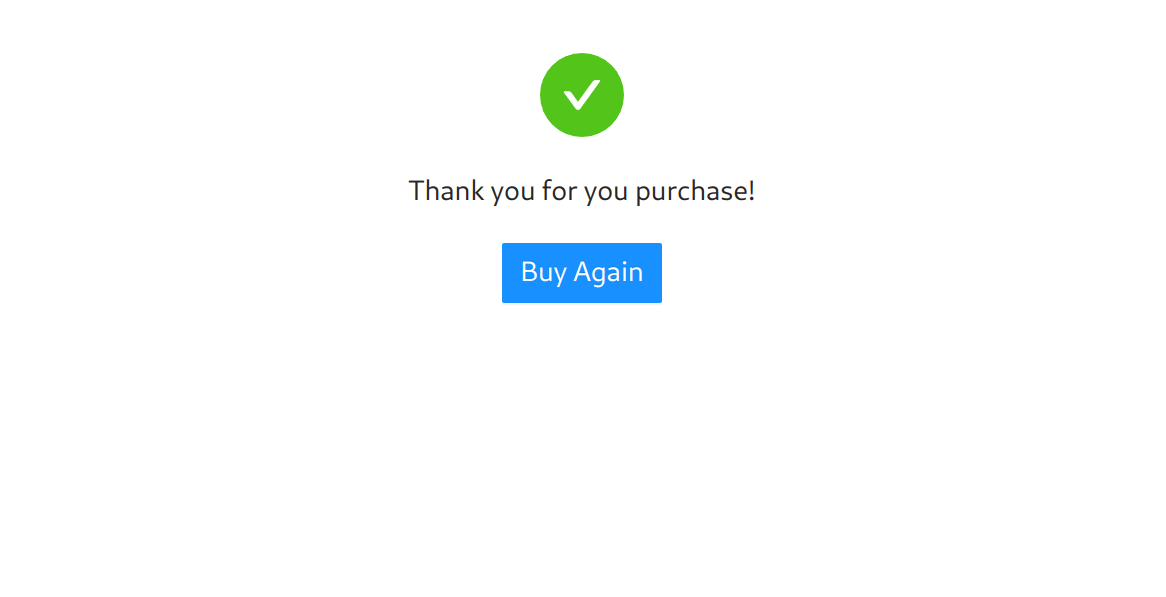
\includegraphics[width=1\textwidth]{./images/userapp5.png}
    \fonte{}
\end{figure}
